\chapter{Videojuegos de Rol}
\label{cap:videojuegosrol}

\begin{resumen}
En este capítulo se explicará qué son los videojuegos, haciendo un enfoque en los videojuegos de rol, se introducirá su historia y se hablará del proceso de desarrollo de estos, analizando la importancia de los motores y editores en el desarrollo de videojuegos.
\end{resumen}

\section{¿Qué es un videojuego?}
Definir qué es un videojuego es una tarea bastante complicada, sobre todo teniendo en cuenta los matices con los que se puede definir (académicos, de diseño, experimentales o tecnológicos). Una de las definiciones más acertadas la da \cite{EspositoVJ}, que lo define como \comillas{un \textit{juego} que se \textit{juega} gracias a un \textit{aparato audiovisual}, y que puede estar basado en una \textit{historia}}. El propio \citeauthor{EspositoVJ} se encarga de definir qué es el \textit{juego}, qué es \textit{jugar}, qué es el \textit{aparato audiovisual} y qué es la \textit{historia}.

\smallskip

La diferencia fundamental de los juegos tradicionales frente a los videojuegos es la existencia de ese \textit{aparato audiovisual} (videoconsolas, ordenador, dispositivos móviles) que pueda ofrecer una interacción \comillas{humano-máquina}, ya que es esta interacción recíproca la que hace que los videojuegos sean videojuegos y no otro tipo de entretenimiento multimedia.

\medskip

A la hora de diseñar un videojuego, hay que tener en cuenta tres conceptos importantes, dos de ellos propuestos por \cite{mda} en su modelo MDA\footnote{El modelo MDA de \citeauthor{mda} intenta cerrar las posibles brechas entre el diseño y el desarrollo de un juego basándose en tres aspectos fundamentales: mecánicas, dinámicas y estética (\textit{\textbf{M}echanics-\textbf{D}ynamics-\textbf{A}esthetics}).}, las mecánicas, las dinámicas y la jugabilidad:
\begin{itemize}
	\item Las \textbf{mecánicas} son las reglas, sistemas y acciones posibles dentro del juego. Incluyen elementos como el movimiento, la recolección de objetos, el combate o el sistema de progresión de los personajes. Se podrían definir como \comillas{los bloques de construcción del juego}.
	\item Las \textbf{dinámicas} son los comportamientos emergentes que surgen de la interacción entre el jugador y las mecánicas, y están estrechamente relacionadas con la experiencia del jugador. Por ejemplo, una mecánica de sigilo puede generar una dinámica de tensión y precaución.
	\item La \textbf{jugabilidad} (o \textit{gameplay}) es la experiencia interactiva del jugador dentro de un videojuego. Pese a que ni \cite{tekinbas2003rules} ni \cite{schell2019art} dan una definición concreta, hablan de cómo la interacción entre el jugador con las reglas del juego y con las mecánicas (es decir, las dinámicas) dan lugar a la jugabilidad. No solo cada juego tiene una jugabilidad distinta que depende de las dinámicas, mecánicas y reglas, sino que puede haber una mecánica emergente que surja a través de las decisiones que cada jugador tome.
\end{itemize}

\medskip

Dependiendo de las mecánicas principales, los objetivos y las formas de interacción que tenga un videojuego, se pueden clasificar en una amplia variedad de géneros.

\smallskip

Los primeros intentos de clasificar los videojuegos mediante características comunes surgen en la década de los 80, principalmente por diseñadores y desarrolladores, como \cite{Crawford84}, quien los categorizó entre aquellos que \textit{requieren de habilidades previas por parte del usuario} (como juegos de combate o de carreras), y \textit{juegos de estrategia} (que engloba al resto de juegos, como los de aventuras, los educativos, y los RPG). Estas categorías son \textit{funcionales}, se centran en las mecánicas de juego y enfatizan cómo los jugadores interactúan con el sistema.

\medskip

Esta categorización ha ido cambiando a lo largo de la historia, hasta llegar a la actualidad, donde los distintos géneros vienen dados por una mezcla de mecánicas, temas, elementos narrativos, estética o lugar de origen y plataforma, y están gravemente influenciados por las tendencias del mercado, discursos mediáticos y la propia percepción de los jugadores. También, muchas veces se quiere categorizar a los videojuegos con etiquetas propias de otras modalidades, como el cine o la literatura, que son incapaces de capturar los aspectos únicos que definen a un videojuego.

\smallskip

Entre esta categorización más \comillas{clásica} se encuentran los siguientes géneros:
\begin{itemize}
	\item Acción, que son todos aquellos juegos que se centran en la velocidad de reacción del jugador y en la coordinación, como por ejemplo juegos de disparos (\textit{shooters}) o plataformas.
	\item Aventura, que prioriza la exploración, la narrativa y, a veces, la resolución de acertijos, como en los juegos \textit{point-and-click}.
	\item Estrategia, que requieren una planificación táctica, ya sea en tiempo real (RTS, \textit{real-time strategy}) o por turnos (TBS, \textit{turn-based strategy})
	\item Simulación, que buscan reproducir aspectos de la vida real, como la gestión de recursos, la conducción de un vehículo o pilotaje de un avión.
	\item Deportes y carreras, que emulan disciplinas deportivas o competiciones de velocidad.
	\item Puzles, que plantean desafíos cognitivos lógicos o espaciales.
	\item Rol, que atendiendo a la definición dada en el capítulo \ref{cap:juegosrol}, son todos aquellos juegos que permitan a sus usuarios encarnar el rol de uno o varios personajes en un mundo ficticio, donde puedan tomar decisiones, interactuar con su entorno y desarrollar una narrativa para conseguir un determinado objetivo.
\end{itemize}

\medskip

\figura{Bitmap/botw}{width=0.7\textwidth}{fig:botw}{Escena de juego de \cite{BOTW}, extraída de \cite{BOTWForbes}.}

\cite{FailGeneros} argumentan que las categorías existentes a día de hoy se quedan cortas para satisfacer los propósitos del género en videojuegos (identidad, agrupación, \textit{marketing} y educación), ya que dada la gran diversidad de juegos que hay ahora, resulta casi imposible poder agrupar la naturaleza multifacética de estos en etiquetas tan \comillas{tradicionales}.

\smallskip

El ejemplo más claro se ve en uno de los juegos más exitosos de la última década, \citegame{The Legend of Zelda: Breath of the Wild}{BOTW}, que mezcla elementos de libre exploración (lo que lo convertiría en un \textit{sandbox} o \comillas{juego libre}), como bien se puede apreciar en la figura \ref{fig:botw} por el enorme mundo en el que se desarrolla la acción; acción en tiempo real e investigación y resolución de rompecabezas (lo que lo convertiría en un juego de \comillas{acción-aventura}); y la progresión en tiempo real del personaje característica de los RPG (se puede ir consiguiendo nuevas habilidades o mejorando el equipamiento). Es por eso que muchas veces hay géneros intermedios, como en este caso, que se podría considerar a \textit{Breath of the Wild} como un RPG de acción (ARPG, \textit{action role-playing game}), que igualmente siguen sin englobar a la increíble diversidad de juegos. Este problema también se puede aplicar a la inversa, donde juegos como \citegame{Undertale}{Undertale}, esencialmente un RPG, tiene elementos, como el combate, propios de otro género de juegos.

\medskip

Hay muchas formas de evitar este problema, y quizá la mejor solución sea dejar de considerar a los géneros como \comillas{cajones estancos} en los que un videojuego no pueda pertenecer a dos de estas categorías simultáneamente \citep{Apperley}, sino que sean más bien un espectro, sin fronteras establecidas, en el que un videojuego pueda caer entre dos categorías distintas.

\smallskip

En resumen, antes de categorizar un videojuego en según qué género, hay que entender que resulta imposible que este se reduzca a una fórmula fija, sino que hay que entenderlo como una combinación fluida de mecánicas, elementos narrativos, temas y estética, que varían de juego a juego.

\subsection{Historia de los videojuegos de rol}

\figura{Bitmap/dnd1975}{width=0.6\textwidth}{fig:dnd1975}{Interfaz de \cite{dnd}, extraída de \cite{dndimage}.}

Es a mediados de la década de los 70 cuando se puede hablar del nacimiento de los videojuegos de rol. Dadas las limitaciones tecnológicas de la época, los RPG primitivos no eran más que simples adaptaciones de juegos de mesa ya existentes por entonces, como \citegame{dnd}{dnd}, una adaptación del anteriormente mencionado \textit{Dungeons \& Dragons}, de donde se tomó su sistema de combate e historia; y posteriormente, en juegos más modernos, se ha tomado el \textit{sistema d20}, las estadísticas de los personajes, o los sistemas de niveles. 

\smallskip

Estos primeros juegos contaban con interfaces basadas en texto, resaltadas con colores muy vivos, y pocos \textit{sprites}, muchas veces llegando a dibujarlos utilizando caracteres ASCII (ver figura \ref{fig:dnd1975}), y normalmente estaban programados en los grandes ordenadores que se encontraban en campus universitarios como los de Harvard o la Universidad de Illinois. Esta primera etapa, \cite{barton2008dungeons} la denomina como la etapa de \comillas{años oscuros}\footnote{En un símil con los años oscuros del Medievo europeo, ya que es un período caracterizado por la falta de literatura e historia escritas y por una decadencia constructiva y cultural.}, ya que es escasa la información que hay hoy en día sobre estos juegos, autores o desarrollo, ya que muchos no se han conservado y se consideran \textit{lost media}, es decir, materiales multimedia que ya no existen en ningún formato y para los cuales no hay ninguna copia disponible.

\smallskip

\begin{figure}[t]
\centering
\begin{SubFloat}
{\label{fig:rogue}%
	Captura de \cite{rogue}, extraída de \cite{rogueimg}}%
	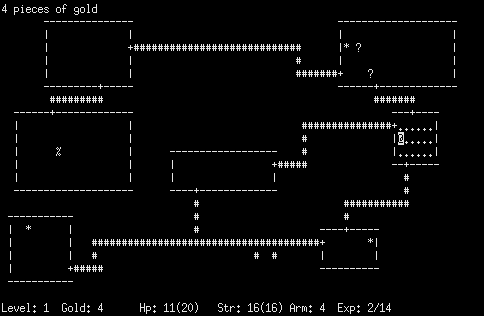
\includegraphics[width=0.45\textwidth]{Imagenes/Bitmap/rogue}%
\end{SubFloat}
\qquad
\begin{SubFloat}
{\label{fig:ultima}%
	Captura de \cite{ultima}, extraída de \cite{ultimaimg}}%
	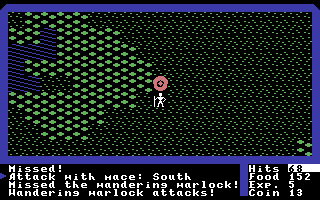
\includegraphics[width=0.45\textwidth]{Imagenes/Bitmap/ultima}%
\end{SubFloat}
\caption{Capturas de \textit{Rogue} y \textit{Ultima}. \label{fig:rogueultima}}
\end{figure}

De esta primera etapa también cabe mencionar tres videojuegos que dieron comienzo a tres distintos subgéneros dentro de los RPG: 
\begin{itemize}
\item \citegame{Rogue}{rogue}, que dio lugar a los videojuegos de mazmorra o \textit{roguelikes}, caracterizados por la generación aleatoria de un laberinto o mazmorra (ver figura \ref{fig:rogue}) en el que se desarrolla una aventura basada en turnos. En este tipo de juegos la muerte es permanente, y al perder la partida se empieza en una nueva desde cero. 
\item \citegame{Wizardry}{wizardry}, que dio lugar a los videojuegos de exploración de mazmorra o \textit{dungeon crawlers}, similares a los anteriores, pero centrados en la exploración de la mazmorra, con un énfasis en la progresión de los personajes y de la gestión de la \textit{party} o escuadrón (el conjunto de personajes que juntos intentan alcanzar objetivos comunes). 
\item \citegame{Ultima}{ultima}, que dio lugar a los RPG de mundo abierto. En esta clase de juegos, los jugadores pueden explorar libremente ciudades, mazmorras, bosques y otro tipo de entornos, manteniendo las mecánicas tradicionales de otros RPG (ver figura \ref{fig:ultima}). 
\end{itemize}

\medskip

Con el salto tecnológico que hubo a mediados de la década de los 80, los RPG comienzan a separase cada vez más de ser meras adaptaciones de juegos ya existentes a desarrollar sus propias historias. A partir de esta época se pueden encontrar dos corrientes bastante diferenciadas de RPG, los \comillas{occidentales} (WRPG, \textit{Western role-playing game}), con más libertad de decisión para los jugadores tanto en personalización como en la historia, y con temáticas realistas (como los anteriormente mencionados \textit{Rogue}, \textit{Wizardry} y \textit{Ultima}); y los \comillas{orientales} o \comillas{japoneses} (JRPG, \textit{Japanese role-playing game}, por ser Japón el país que más videojuegos de este tipo produce), centrados en una narrativa lineal con temáticas fantásticas y mecánicas basadas en turnos. Dos grandes videojuegos que definieron el género de los JRPG son \citegame{Dragon Quest}{dq} y \citegame{Final Fantasy}{ff}, cuyas sagas permanecen hasta la actualidad con nuevas entregas cada pocos años. Son estos años de apogeo de los RPG los que \citeauthor{barton2008dungeons} denomina como \comillas{etapa dorada}.

\medskip

La década de los 90 supuso un grave declive para los RPG, especialmente en los mercados occidentales, ya que la aparición de juegos de acción en 3D, como \citegame{Doom}{doom}, \citegame{Quake}{quake} o \citegame{Tomb Raider}{lc}, hizo que el mercado cambiase hacia este tipo de juegos, mucho más rápidos y frenéticos que los RPG, que se consideraban obsoletos, con una pesada carga textual y mucho más lentos de jugar. También, la aparición de videoconsolas mucho más potentes y baratas, como la \textit{PlayStation} (Sony, 1994) o la \textit{Nintendo 64} (Nintendo, 1996), para las cuales los RPG occidentales no tenían portabilidad\footnote{Son muchas las decisiones por las cuales las empresas \comillas{occidentales} no quisieron portar sus juegos hacia las nuevas consolas, como por ejemplo las limitaciones que iba a suponer (algunos requerían teclado y ratón), los altos costes que conllevaba el rediseño de muchos de los juegos y la poca demanda que se consideraba que los juegos iban a tener en estas plataformas.}, y los altos costes de desarrollo y producción que supuso el cambio de cartuchos tradicionales a nuevos formatos como CD-ROM, hicieron que los RPG, especialmente los WRPG, tuviesen este gran declive que solo pudo recuperarse a mediados de la siguiente década.

\medskip

En el nuevo milenio, que para \citeauthor{barton2008dungeons} es la \comillas{etapa de platino}, surgen sagas con juegos con gráficos mucho más sofisticados y con narrativas mucho más profundas, como la saga \textit{The Elder Scrolls}, más concretamente, su tercera entrega, \citegame{Morrowind}{tes}; la saga \citegame{Fallout}{fallout}; la saga \citegame{Baldur's Gate}{baldurs}; o la saga \citegame{Diablo}{diablo}, que llevan hasta el límite las propias definiciones del género por las mezclas con otros géneros (llegando a ser juegos \comillas{híbridos}). La potencia del \textit{hardware} va en aumento, lo que permite que haya un salto cualitativo, tanto gráfico como en jugabilidad, mientras que la tendencia de los mundos abiertos continúa y se mejora, llegando a ser algunos RPG como \citegame{The Elder Scrolls V: Skyrim}{skyrim} o \citegame{The Witcher 3: Wild Hunt}{witcher} los más vendidos.

\section{Sobre el desarrollo de videojuegos}
Para entender cómo, bien las empresas profesionales o bien equipos \textit{indies} desarrollan un videojuego desde cero, es imprescindible saber con exactitud cómo funciona el software internamente, y qué formas tienen los programadores o desarrolladores para comunicarse con las entrañas de este durante el proceso de desarrollo. Es por eso que en este apartado se explicará qué es un \textit{motor} y qué es un \textit{editor}.

\subsection{Roles en el desarrollo de videojuegos}
El desarrollo de un videojuego es una tarea multidisciplinar que requiere la colaboración de múltiples individuos expertos en múltiples áreas. Por lo general, los roles más comunes dentro de un equipo de desarrollo profesional\footnote{En proyectos pequeños o empresas \textit{indies} estas funciones pueden solaparse, ya que no siempre se puede contar con expertos en todas las materias.} son los siguientes:
\begin{itemize}
	\item \textbf{Diseñador}: es el responsable de definir las mecánicas del juego, las reglas, los objetivos, la progresión y la experiencia general del jugador. También se encarga del diseño de los niveles, de los sistemas de juego o del equilibrio de la dificultad.
	\item \textbf{Programador}: se encarga de implementar técnicamente el videojuego utilizando lenguajes de programación y motores de desarrollo. Es común que haya programadores especializados en distintas áreas, como la inteligencia artificial, gráficos, físicas o red.
	\item \textbf{Artista}: se encarga de diseñar los elementos visuales del juego, como personajes, escenarios, animaciones y efectos visuales. Dependiendo del estilo del juego, puede haber artistas 2D, 3D, conceptuales ({\textit{concept artist}}) o de interfaces.
	\item \textbf{Diseñador de sonido}: se encarga del diseño y producción de los efectos de sonido, música y ambiente del juego. A menudo colabora con compositores y actores de voz para dotar de identidad sonora al juego.
	\item \textbf{Guionista}: se encarga de crear la historia, los diálogos, el trasfondo y el desarrollo narrativo del juego. Es fundamental en aquellos géneros donde la narrativa tiene un peso importante, como es el caso de algunos RPG.
	\item \textbf{Probador}: su misión es detectar errores, evaluar la jugabilidad y asegurar que el producto final funcione correctamente. Esta fase se conoce comúnmente como QA (\textit{quality assurance}, aseguramiento de la calidad), y es esencial para garantizar una buena experiencia de usuario.
	\item \textbf{Productor}: se encarga de coordinar al equipo, gestionar los tiempos, recursos y comunicación entre los distintos departamentos. Es el vínculo entre el equipo creativo y las partes interesadas externas (como clientes, editoras o inversores).
	\item \textbf{Director creativo}: supervisa la visión general del juego y asegura que todos los elementos (jugabilidad, arte, narrativa...) estén alineados con el concepto original.
\end{itemize}

\subsection{Motor de videojuegos}
\cite{gregory2018game} define un motor de videojuegos (\textit{game engine}) como \comillas{todo aquel \textit{software} extensible que, sin apenas modificaciones, puedan servir de base o cimiento para múltiples videojuegos distintos}. Este \textit{software} es todo el conjunto de herramientas que hacen que por detrás funcione un juego, como por ejemplo, todas las herramientas que se encarguen del \textit{renderizado} o dibujado en pantalla, bien sea en 2D o en 3D, aquellas que se encarguen de la simulación física y detección de colisiones con el entorno, las que se encarguen del sonido, las del \textit{scripting}, animaciones, inteligencia artificial\ldots A todas estas herramientas también se les denomina \textit{motores} (por ejemplo, \textit{motor de render}, \textit{motor de físicas}\ldots).

\smallskip

Estos \textit{motores de tecnología} conforman la infraestructura básica técnica del motor más complejo que las usa, y se usan para abstraer la interacción con el \textit{hardware} o sistema operativo; por lo que un motor de videojuegos también podría describirse como \comillas{una capa de abstracción y herramientas orientadas al desarrollo de videojuegos elaborada sobre \textit{motores de tecnología}}.

\medskip

Debido a las limitaciones tecnológicas de los años 70 y principios de los 80, los primeros juegos se desarrollaban todos desde cero, sin apenas compartir código un juego con otro, ya que cada uno necesitaba una lógica optimizada de una determinada manera que otros no necesitaban o no podían utilizar. Además, los juegos solían ser lanzados para una única plataforma, ya que portar un juego a otra distinta con otra serie de requisitos y limitaciones implicaba reescribirlo desde cero, y muchas veces los desarrolladores eran equipos muy pequeños (llegando a ser incluso de una única persona) y no todas las grandes empresas disponían de departamentos de portabilidad.

\smallskip

No es hasta mediados y finales de la década de los 80 cuando los desarrolladores comienzan a reutilizar código entre juegos y surgen los primeros ejemplos de lo que hoy se podría llamar \comillas{motor}. Uno de los primeros fue el que Shigeru Miyamoto desarrolló en Nintendo para la \textit{Nintendo Entertainment System} (según explica \cite{williams2017history}), que se utilizaría en juegos como \citegame{Excitebike}{excitebike} o \citegame{Super Mario Bros.}{smb}.

\smallskip

A principios de los 90 surgen los primeros \comillas{motores modernos}, de la mano de desarrolladoras como \textit{id Software} y juegos como \textit{Doom} o \textit{Quake}, quienes decidieron reutilizar toda la lógica de \textit{renderizado} y los sistemas de simulación física, ya que cada parte estaba desarrollada de manera independiente. Tal fue el éxito que alcanzaron estos dos juegos que muchas empresas prefirieron pagar a \textit{id Software} por una licencia del núcleo del motor y diseñar sus propios recursos, que desarrollar su propio motor desde cero. Una de estas empresas fue \textit{Valve}, quienes desarrollaron uno de los mejores juegos de la historia, \citegame{Half-Life}{hl}, utilizando el motor \textit{GoldSrc} (que es el antecesor del actual motor de Valve, \textit{Source}), una versión modificada del motor de \textit{id Software}.

\medskip

Con la generalización de internet a principios de los 2000, comenzó el auge de comunidades de \textit{modding} en línea, y muchas desarrolladoras comenzaron a lanzar motores de código abierto acompañados por editores de niveles o herramientas de \textit{scripting} (es decir, código de alto nivel, normalmente no compilado, que solo modifica lógica del juego o eventos sin modificar el núcleo del motor).

\smallskip

A día de hoy, las empresas dedican numerosos recursos a la hora de desarrollar nuevos motores, ya que son la parte fundamental del desarrollo de videojuegos, y cada vez son más sofisticados y requieren de un gran conocimiento en programación o en diseño.

\smallskip

Los desarrolladores \textit{indie}, por su parte, tienen la posibilidad de poder desarrollar sus propios motores, cuyo contenido no es equiparable al de empresas que producen juegos \textit{triple A} (aquellos juegos producidos por grandes empresas a los que se suelen destinar un alto presupuesto en desarrollo y publicidad); usar motores propietarios de empresas con licencias gratuitas o de poco coste, como por ejemplo \textit{Unity} o \textit{Unreal Engine}; o motores de código abierto, como \textit{Godot}. Por lo general, estos motores suelen venir acompañados de un editor, que facilita el desarrollo de los juegos implementados para ese motor.

\subsubsection{Componentes de un motor de videojuegos}
\begin{figure}[t]
	\begin{center}
		\begin{tikzpicture}[enginebox/.style={draw, thick, minimum width=9cm, minimum height=6cm, align=center},
  subbox/.style={draw, thick, minimum width=3.8cm, minimum height=1cm, align=center},
  labelbox/.style={draw, thick, minimum width=3cm, minimum height=1cm, align=center}]
  			\node[labelbox] (game) {\textbf{Juego}};
	
			\node[enginebox, below=1.5cm of game] (engine) {\textbf{Motor}};
	
			\node[subbox, anchor=north west] at ([xshift=0.5cm, yshift=-0.3cm]engine.north west) (render) {Motor de \textit{render}};
	
			\node[subbox, right=0.5cm of render] (physics) {Motor de físicas};
	
			\node[subbox, below=0.3cm of render] (sound) {Motor de sonido};
	
			\node[subbox, right=0.5cm of sound] (input) {Motor de \textit{input}};
	
			\node[subbox, below=2.1cm of render] (net) {Motor de red};
	
			\node[subbox, right=0.5cm of net] (scripting) {Motor de \textit{scripting}};
	
			\node[subbox, below=0.3cm of net] (anim) {Sistema de animación};
	
			\node[subbox, right=0.5cm of anim] (AI) {Motor de IA};
	
			\draw[->, thick] (game.south) -- node[midway, right] {utiliza} (engine.north);
		\end{tikzpicture}
		\caption{Representación esquemática de la estructura de un juego y su motor con algunos de los componentes principales} 
		\label{fig:juegoymotor}
	\end{center}
\end{figure}

Cada motor de videojuegos es distinto, y cada uno incorpora según qué motores de tecnología dependiendo de las necesidades de los programadores o del juego que se esté programando. Siguiendo el esquema provisto en la figura \ref{fig:juegoymotor}, estos son los componentes principales de un motor de videojuegos tanto de grandes empresas, como motores con licencia gratuita, como aquellos de código abierto:
\begin{itemize}
\item \textbf{Motor de render o de dibujado}: se encarga de gestionar todas las tareas relacionadas con los gráficos que se muestran en pantalla. Para ello, dibuja objetos bidimensionales o tridimensionales, representados generalmente mediante \comillas{mallas}, a través de técnicas de informática gráfica, como pueden ser la \textit{rasterización} o el trazado de rayos. También es el encargado de gestionar la cámara, luces, sombras, materiales y texturas, y puede aplicar diversos efectos de posprocesado al fotograma final. Muchas de estas tareas las puede definir el propio programador haciendo uso de un tipo de \textit{script} especial llamado \textit{shader}, que en lugar de ejecutarse en el procesador de un ordenador se ejecuta en el procesador de las tarjetas gráficas. Estos motores suelen ser una capa de abstracción sobre especificaciones estándar para gráficos como \textit{OpenGL}, \textit{Vulkan}, \textit{DirectX} o \textit{Metal}.
\item \textbf{Motor de físicas}: se encarga de simular comportamientos físicos realistas. Entre estos comportamientos físicos se encuentran las colisiones de objetos con otros objetos o con el entorno, aplicar la fuerza de gravedad a unos determinados objetos, simular las dinámicas de cuerpos rígidos (es decir, el movimiento de cuerpos interconectados bajo la acción de una fuerza externa, como por ejemplo, cajas que se pueden tirar, deslizar o romper), simular dinámicas de cuerpos blandos (similares a los cuerpos rígidos, pero con la posibilidad de que estos se deformen), y, en algunos casos, simulaciones de fluidos y de materiales textiles. Ya que hacer una simulación física es complicado, se suelen utilizar motores de terceros, como por ejemplo \textit{NVIDIA PhysX}, \textit{Havok}, \textit{Bullet} o \textit{Box2D}.
\item \textbf{Motor de sonido}: se encarga de gestionar los efectos de sonido, la música, el audio espacial o posicional en dos o tres dimensiones, y todos los efectos sonoros que se pueden aplicar al sonido (reverberación, eco, tono, barrido, mezclado de pistas, oclusión sonora, efecto Doppler, etc\ldots). Algunas librerías utilizadas son \textit{FMOD}, \textit{OpenAL}, \textit{Wwise} o \textit{irrKlang}.
\item \textbf{Motor de \textit{input} o de gestión de la entrada}: se encarga de capturar y procesar eventos de entrada (\textit{input}) del usuario a través de los diversos dispositivos para los que se programe (teclado y ratón, mandos o controladores y pantallas táctiles) y asociarlos a las acciones definidas en el juego.
\item \textbf{Sistema de animación}: gestiona animaciones de \textit{sprites} (los elementos gráficos bidimensionales básicos que representan visualmente objetos dentro del juego) o de esqueletos (\textit{rigging}, usados para personajes tridimensionales). Suelen tener soporte para árboles de mezcla y cinemática inversa.
\item \textbf{Motor de \textit{scripting}}: permite escribir lógica específica del juego utilizando lenguajes de programación de alto nivel (como por ejemplo JavaScript, Lua, C\# o Python), separando la implementación de la jugabilidad de la implementación del motor. El \textit{scripting} se suele hacer mediante lenguajes de programación interpretados y no compilados, por lo que los cambios más pequeños no requieren volver a iterar por todo el proceso de compilado del motor o del juego.
\item \textbf{Motor de red}: se encarga de gestionar el soporte multijugador, es decir, la comunicación y sincronización cliente-servidor o cliente-cliente. El motor de red también incluye sistemas de emparejamiento (\textit{matchmaking}) y de predicción o interpolación del juego para una simulación fluida en los juegos multijugador.
\item \textbf{Motor de inteligencia artificial}: ofrece herramientas para poder crear comportamientos inteligentes artificiales, como por ejemplo, algoritmos de búsqueda de caminos (\textit{pathfinding}, como los algoritmos \textit{A*} o el de Dijkstra), árboles de comportamiento y máquinas de estado, o sistemas de toma de decisiones. Este motor suele tener una conexión directa con el motor de \textit{scripting} para poder definir comportamientos mucho más fácilmente.
\item \textbf{Gestor de recursos}: maneja la carga y descarga de recursos como texturas, mallas, sonidos o animaciones, muchas veces bajo demanda del juego mediante gestores de memoria, compresión y de transmisión de datos altamente optimizados.
\item \textbf{Sistema de interfaz de usuario}: se encarga de gestionar la barra de estado (HUD, \textit{head-up display}), los menús, texto, botones y otros elementos de la interfaz con los que el usuario pueda interactuar.
\end{itemize}

\subsubsection{Separación entre motor y \textit{gameplay}}
\begin{figure}[t]
\centering
\begin{SubFloat}
	{\label{fig:separaciongeneral}%
		Separación en motores generalistas.}%
		\begin{tikzpicture}
		\draw (0,0) rectangle (3,6);
		\draw[red, dashed] (-1,2) -- (4, 2);
		\node at (1.5,4) {\textit{Gameplay}};
		\node at (1.5,1) {Motor};
		\end{tikzpicture}
\end{SubFloat}
\qquad
\begin{SubFloat}
	{\label{fig:separacionespecificos}%
		Separación en motores específicos.}%
		\begin{tikzpicture}
		\draw (0,0) rectangle (3,6);
		\draw[red, dashed] (-1,4) -- (4,4);
		\node at (1.5, 5) {\textit{Gameplay}};
		\node at (1.5, 2) {Motor};
		\end{tikzpicture}
\end{SubFloat}
\caption{Ejemplos de separaciones entre motor y \textit{gameplay} en los distintos motores. \label{fig:separacionesmotgp}}
\end{figure}

Para poder reusar un motor en múltiples juegos con el menor número de cambios, es necesario saber \textit{cómo y para qué vamos a desarrollar el motor}, y de acuerdo a la decisión que se haya tomado, se establecerá la barrera de separación entre el motor y la jugabilidad del juego.

\medskip

Los motores más generalistas, como los anteriormente mencionados \textit{Unity}, \textit{Unreal Engine} o \textit{Godot}, debido a que están pensados para poder ejecutar todo tipo de juegos, tienen una barrera de separación entre el motor y el \textit{gameplay} que se suele establecer a la mitad. La implementación del juego final que tienen este tipo de motores es mínima (el motor es puramente un conjunto de \textit{motores de tecnología}) y es el desarrollador, o a veces el diseñador\footnote{En muchos casos, hay veces que los propios diseñadores también pueden implementar parte del juego sin la necesidad de tener conocimientos de programación. Para ello, existen los editores, que se explicarán en la sección \ref{sec:editorvj}.}, el que se tiene que encargar del desarrollo de la jugabilidad. En la figura \ref{fig:separaciongeneral} se puede ver esta \comillas{separación} de manera esquemática, donde la parte de la jugabilidad es mucho más amplia que la del motor, que solo incluye elementos básicos para que un juego funcione. 

\smallskip

La gran ventaja que tienen los motores generalistas frente a los específicos es la libertad que dejan al desarrollador (o diseñador) para poder implementar la jugabilidad a su manera, con las reglas y mecánicas que se hayan establecido previamente.

\medskip

En el caso de aquellos motores que fijan gran parte de la jugabilidad de los juegos que se puedan hacer con ellos, y que lo único modificable son algunos parámetros del \textit{gameplay} y las partes artísticas y visuales, se tendrán que introducir elementos propios del juego en el motor, dejando menos libertad de implementación en el \textit{gameplay}. En la figura \ref{fig:separacionespecificos} se aprecia cómo la barrera de separación entre la implementación del juego que contiene el motor frente a la de la jugabilidad es mucho más alta que en la figura \ref{fig:separaciongeneral}, por lo que el motor ya no solo incluirá elementos básicos para el funcionamiento del juego, sino elementos específicos de un tipo de juego en concreto.

\smallskip

Este tipo de motores son mucho más rígidos a la hora de poder implementar nuevas funcionalidades y limitan bastante los juegos que se pueden crear con ellos, pero simplifican bastante el desarrollo, y son especialmente útiles para nuevos programadores.

\subsubsection{Programación dirigida por datos (DDP) en videojuegos}
La programación dirigida por datos (DDP, \textit{data-driven programming}) es un paradigma de diseño en el que gran parte del comportamiento y lógica de un programa están controlados por datos externos en lugar de estar programados en el código fuente de este. Este paradigma, según \citeauthor{gregory2018game}, ampliamente extendido entre las empresas desarrolladoras de juegos \textit{triple A}, permite a los desarrolladores modificar o expandir el comportamiento del juego sin la necesidad de alterar el motor o el código base de este.

\medskip

Los motores de videojuegos suelen estar programados utilizando lenguajes de \textit{medio nivel}\footnote{Los lenguajes de \textit{nivel medio}, como C o C++, serían aquellos lenguajes de alto nivel que proporcionan estructuras de acceso a \textit{hardware} como los lenguajes de bajo nivel.}, ya que se espera poder optimizar al máximo el programa, así como poder tener un soporte multiplataforma. De todo el gran abanico de lenguajes de nivel medio, un gran porcentaje son lenguajes compilados, es decir, requieren de un \comillas{traductor} (compilador) para generar el código máquina antes de poder ejecutar el programa. Esta compilación depende del tamaño del proyecto y del número de ficheros a compilar, y, en el caso de muchos motores, la compilación puede llegar a tardar decenas de minutos.

\smallskip

Para evitar tener que esperar estos minutos recompilando todo un juego en caso de cambiar un simple parámetro referente al \textit{gameplay}, se opta por la solución más flexible, que es desarrollar todo el juego utilizando datos, generalmente en lenguajes de \textit{scripting}, de alto nivel, como Lua, que no necesitan ser compilados, sino interpretados (la \comillas{traducción} a lenguaje máquina se realiza en ejecución del programa y a medida que sea necesaria) por el motor del juego.

\medskip

Además de reducir los tiempos de compilación en los juegos, lo cual ayuda a reducir los tiempos en las iteraciones de desarrollo, la programación dirigida por datos permite a los diseñadores del juego, que no tienen que ser necesariamente programadores, modificar comportamientos, ajustar parámetros o añadir contenido utilizando archivos de configuración o mediante herramientas visuales.

\medskip

Este paradigma refuerza la ya mencionada separación entre motor y \textit{gameplay}, ya que un mismo motor puede ejecutar distintos juegos (es decir, distintos datos) sin la necesidad de tener que ser recompilado, siempre y cuando los datos estén en un formato y estructura que el motor sea capaz de interpretar.

\medskip

Sin embargo, uno de los principales problemas que supone este paradigma es la depuración del código. Como los datos se suelen almacenar en lenguajes de \textit{scripting}, o en lenguajes de almacenamiento de datos (como JSON o XML), depurar un código o simplemente datos que nuestro motor interpretan, resulta extremadamente difícil si el motor no cuenta con herramientas de depuración integradas específicas para interpretar esos datos.

\subsubsection{Programación multiplataforma en videojuegos}

\subsection{Editor de videojuegos} \label{sec:editorvj}

\subsubsection{Editores específicos de videojuegos para desarrollo de RPG}

